\section{Introduction}
\label{sec:intro}

As computing platforms migrate towards clusters of increasingly larger scale of microprocessors,
 applications need to manage the distributed memories of the processors via explicit
message-passing runtimes, for example, MPI, to attain high performance.
The relative latency and bandwidth of the communication network in relation to the compute capacity of processors
are often hard to predict a priori and may change dramatically from one system to the next.
Even on supercomputers comprised of homogeneous nodes,
system noise is increasing on each node because of aspects such as power management, deeper memory hierarchies, and sharing of hardware such as caches and network. The ``equal work means equal time" paradigm is no longer relevant on most systems, and load imbalance increasingly becomes the common scenario even on applications that are symmetrically structured.
Consequently, bulk-synchronous communication, where all processes synchronize frequently, is no longer a valid option for high performance MPI applications.
Application performance is often critically determined by its ability to flexibly overlap communications with local computations,
thereby minimizing wait time.


This paper aims to automatically enable the use of nonblocking latency-hiding techniques to overlap local computation with remote communication in MPI applications, thereby enhancing their overall efficiency and performance portability.
%through a framework that systematically combines analytical performance modeling of the application execution flow and compiler-assisted safety and profitability analysis.
To illustrate the optimization, Figure~\ref{fig:ft_loop} shows the
structure of the NAS FT benchmark~\cite{npb}, which applies fast
Fourier transform (FFT) to a 3D matrix through a loop that interleaves
the computation of scaling the input matrix with a collective
communication of MPI\_Alltoall to exchange data among the
processes. This is then followed by a final transposition of the
resulting matrix.  The clear separation of computation and
communication phases makes the algorithm design easy to implement and
maintain.  Additionally, the communication buffers can be reused
across different loop iterations, saving memory.  However, the
blocking MPI communication requires that all processes wait while the
MPI\_Alltoall operation is in progress.  Consequently, unless the
application is executed on a platform with the fastest network
connections, its performance is likely to suffer because of the
excessive wait time.

\begin{figure}
  \centering
  \begin{subfigure}[b]{0.2\textwidth}
    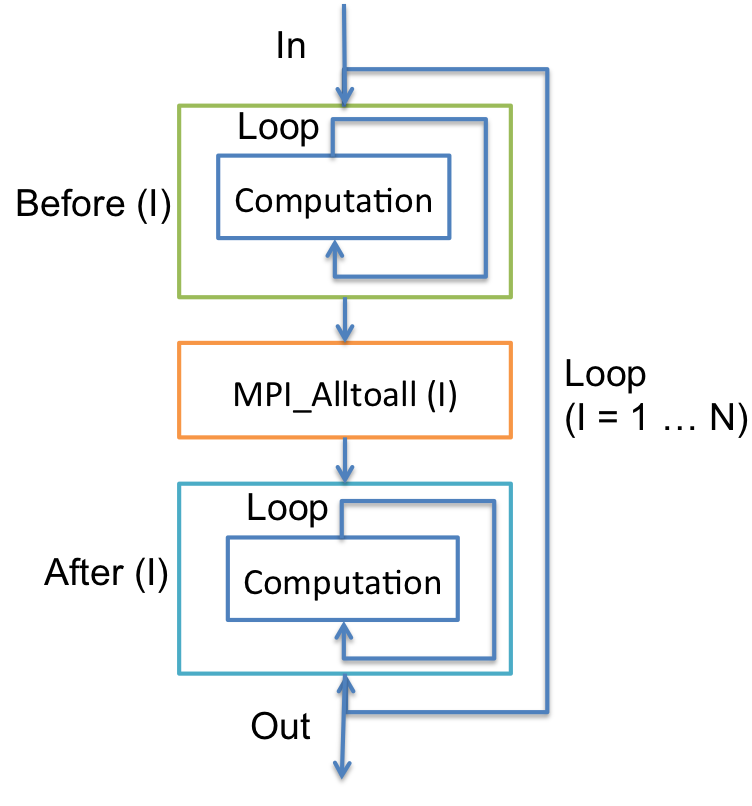
\includegraphics[width=0.8\textwidth,height=1.8in]{fig/ft_loop.png}
    \caption{Before optimization}
    \label{fig:ft_loop}
  \end{subfigure}%
  \hspace{-.3in}
  \begin{subfigure}[b]{0.3\textwidth}
    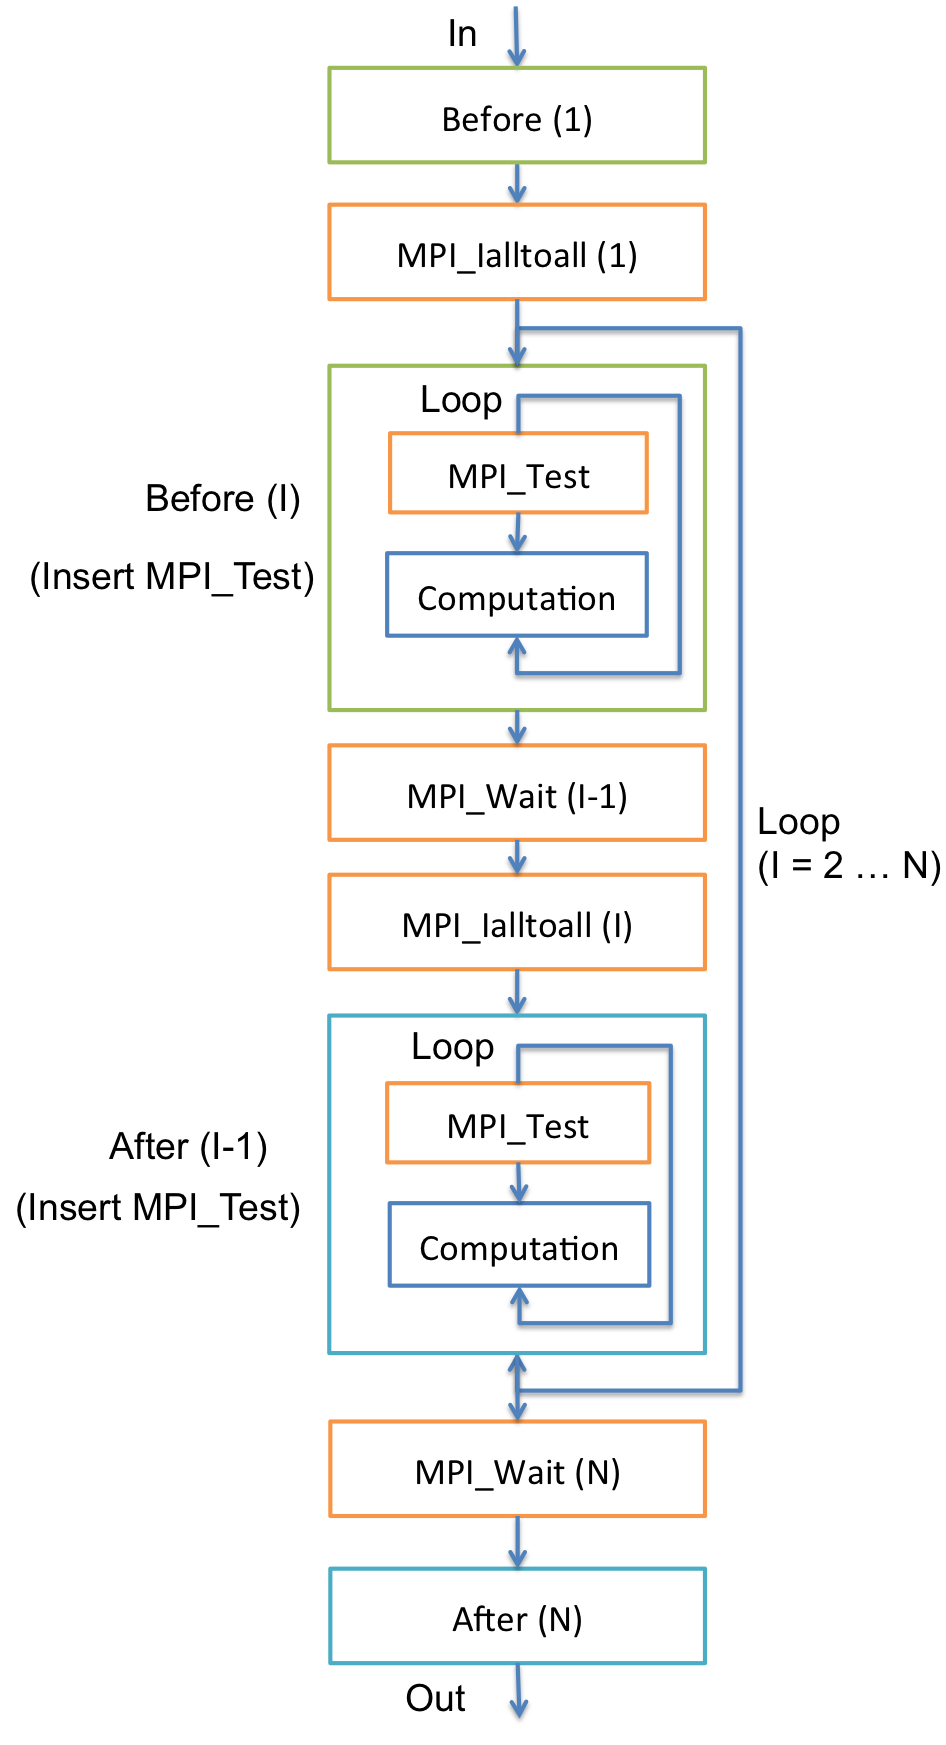
\includegraphics[width=1.1\textwidth,height=1.8in]{fig/ft_cco.png}
    \caption{After optimization}
    \label{fig:ft_cco}
  \end{subfigure}
  \caption{Structure of NAS FT (1D layout) before (a) and after (b)
    overlapping computation and communication.  \emph{Before} and
    \emph{After} in the figures are computation loops before and after
    the communication.}
\label{fig:ft}
\end{figure}

Figure~\ref{fig:ft_cco} illustrates how the structure
in~\ref{fig:ft_loop} may be modified to better overlap computation
with communication.  In particular, the MPI\_Alltoall operation is
decoupled into two finer-grained operations: a nonblocking
MPI\_Ialltoall and a blocking MPI\_Wait.  Then, the loop is modified
so that Before(i), which multiplies a local matrix with a
time-evolution array and then saves a transpose of the matrix into a
local buffer to be communicated to other processors, and
MPI\_Ialltoall(i), which exchanges the local transposes among different
processes, are essentially moved so that they are evaluated before
$MPI\_Wait(i-1)$, which waits for the completion of MPI communication
of the previous iteration, and $After(i-1)$, which processes the just
received remote data (of the $i-1$th iteration), and then print the
result into an output file.  By using two distinct buffers to store
the data used in consecutive MPI communications, the output
dependencoes between After(i-1) and Before(i)/MPI\_Ialltoall(i) can be
eliminated, thereby guaranteeing the correctness of optimization.

Finally, \emph{MPI\_Test} operations are inserted into the local computation to
ensure the progress of the nonblocking
communications.\footnote{Although MPI communications do not need full
  usage of CPU, they need some CPU time, e.g., to manage communication
  progress, which is supplied only when operations such as MPI\_Test
  and MPI\_Wait are invoked.}  By overlapping the MPI communications
with the local computations, the transformed code allows the
application to perform well even on systems with slow network
connections, although nonblocking communications generally take longer
time to finish than blocking ones, and more memory may be needed to
hold the data during communications.

\begin{figure}[h]
\centering
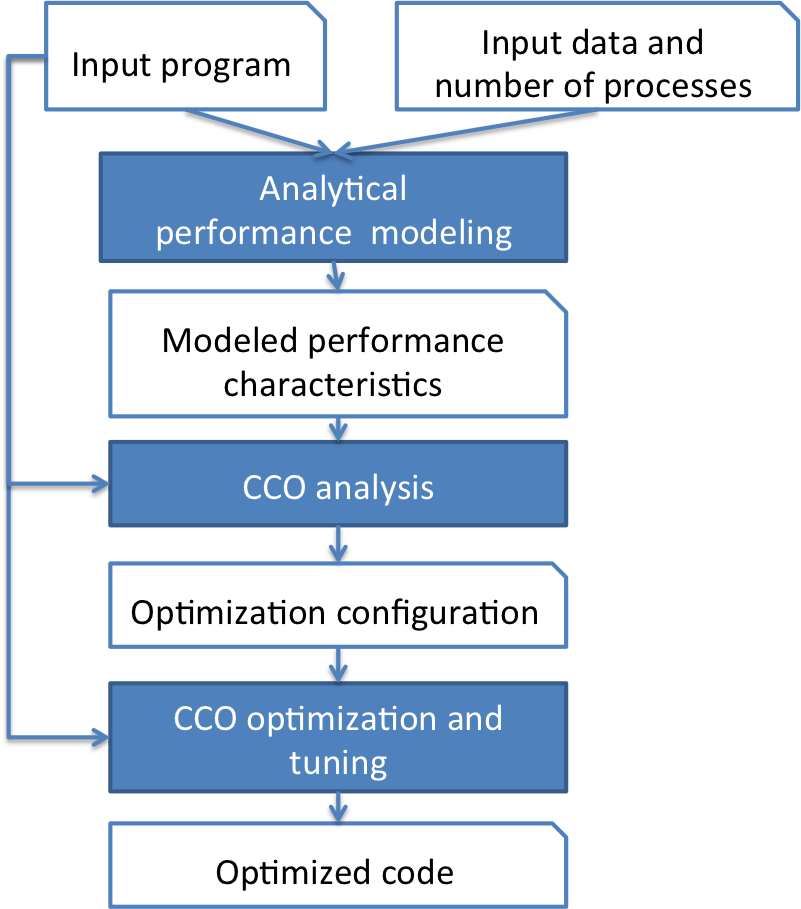
\includegraphics[width=0.35\textwidth]{fig/framework.png} % half page
\caption{Workflow of the CCO optimization approach}
\label{fig:overview}
\end{figure}

Figure~\ref{fig:overview} shows our workflow for systematically
enabling communication-computation overlapping (CCO) in large MPI
applications and thereby enhancing their performance portability.  The
workflow contains three key components: (1) the \emph{performance
  modeling} component, which analyzes the runtime statistics of an MPI
application to extract a {\emph Bayesian execution
  tree\cite{jichi:ipdps14}} representation of its execution flow,
including the frequencies of various runtime code paths and their
performance characteristics such as computation intensities, working
set sizes, and communication characteristics of MPI operations; (2)
the \emph{CCO analysis} component, which identifies {\emph hot}
computation and communication regions that are likely to benefit from
the optimization and summarizes the result of profitability and safety
analysis of the optimizations; and (3) the \emph{CCO optimization and
  tuning} component, which applies the appropriate program
transformations by replacing the blocking MPI operations with
nonblocking ones, by reordering the computations and communications
involved and by inserting MPI\_Test operations with a frequency
determined by empirical tuning of the optimized code.  Note that in
order to guarantee the profitability of the optimization, any
communication slowdown from the use of the nonblocking operations must
be fully overlapped with the local computation, and the insertion of
MPI\_Test operations should cause only marginal slowdown of the local
computation so that its effect is insignificant when compared with the
reduction of the original communication time.  Our framework currently
uses empirical tuning of the optimized code to select appropriate
optimization configurations and to skip nonprofitable optimizations.

The idea of overlapping computation and communication in MPI applications have been
well studied in the past~\cite{danalis:sc05,fishgold:ipdps06}, including both using analytical performance
models~\cite{iancu:ppopp07}
and using compiler analysis~\cite{danalis:ics09} to assist the optimization.
Our work is unique in that it fully integrates both the performance modeling and compiler analysis to collectively
determine both the profitability and safety of the overlapping optimization.
Additionally, it
focuses on a special inter-procedural pattern of loop-based
communication-computation overlapping in scientific applications, which has not been addressed
by existing literature. Our main contributions are the following:

\begin{itemize}

\item We present a framework that integrates analytical performance
  modeling of large MPI applications, semantic inlining of
  developer-supplied domain knowledge, and pattern-based
  transformation in order to systematically enable better overlapping
  of MPI communications with independent local computations to enhance
  the performance portability of MPI applications. We currently
  manually applied the necessary program transformations (the last
  stage of the optimization) but expect to automate this step in our
  future work.

\item We applied our approach to optimize 7 NAS Parallel Benchmarks
  (NPB) applications on both a high-speed and a slow network-connected
  cluster environment and achieved 3--88\% speedup on both platforms.

\end{itemize}

In particular, we use performance modeling to find the candidate hot code paths to optimize.
Comparing to profilers that usually provides measurement for static code blocks,
  our modeling framework also distinguishes dynamic paths involving the same code block,
  which is used to identify the inter-procedural communication pattern.
And then, we use compiler analysis to make sure our optimization will not violate dependence constraints.
Currently we manually applied the optimization transformation for each NPB application,
  because we find these applications to have different MPI communication functions and computation loops,
  which makes it challenging to have a single fully-automatic transformation to work for all NPB applications.

The remainder of the paper is organized as follows.
Section~\ref{sec-model} presents our analytical performance modeling
component for automatically identifying communication and computation
hot spots in MPI applications Section~\ref{sec-analysis} discusses how
to determine the safety of computation-communication overlap through
optimization analysis.  Section~\ref{sec-opt} summarizes strategies we
used to perform the actual optimizations and the tuning of their
configurations.  Section~\ref{sec-exp} evaluates our framework using 9
NAS application benchmarks~\cite{npb}.  Section~\ref{sec-related}
discusses related work, and Section~\ref{sec-concl} presents our
conclusions.
